\section*{Библиотека моделирования потоков}
\addcontentsline{toc}{section}{Библиотека моделирования потоков}
\subsection*{Моделирование потоков}
\addcontentsline{toc}{subsection}{Моделирование потоков}

\textbf{Задание:}\\
Промоделировать процесс производства мороженого. Мороженое производится из молока, сахара и масла в пропорциях 60:10:30. Ингредиенты поступают в реактор-смеситель из резервуаров потрубопроводам -- молоко и сахар, по контейнеру — масло. В смесителе составляющие смешиваются в заданных пропорциях и смесь настаивается10 минут. Далее смесь по трубопроводу поступает в реактор заморозки. Процесс замораживания занимает 10 минут. Полученная смесь порциями по 100 граммов помещается в стаканчики. Стаканчики пакуются по 50 штук. Упаковки мороженого отправляются на склад.\\

\textbf{Решение:}\\
Для начала необходимо создать источники потоков. Источники потоков моделируются блоком \textit{FluidSource}. Для трех источников ингредиентов потребуются 3 подобных блока. \textit{FluidSource} может работать либо как источник с неограниченным объемом, либо как источник с ограниченным начальным объемом, который может наполняться заново вызовом функции inject(). Данный блок задает ограничение на скорость выходного потока, реальная скорость не может превосходить это значение. (Рисунок \ref{fig:fluid1})
\begin{figure}[h]
	\centering 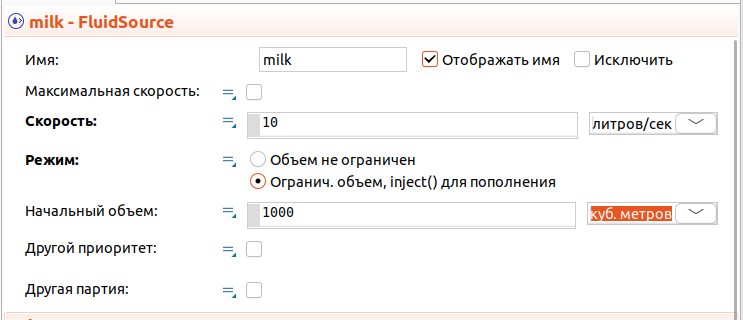
\includegraphics[scale=0.35]{fluid1}
	\caption{Блок источник \textit{FluidSource}}
	\label{fig:fluid1}
\end{figure}

Скорости подачи ингредиентов разные, поэтому понадобятся резервуары для их хранения после того, как они потупили в модель. Резервуары моделируются блоком \textit{Tank}, в котором задаются такие свойства как объем резервуаров и скорости потоков на их выходе. (Рисунок \ref{fig:fluid2})
\begin{figure}[h]
	\centering 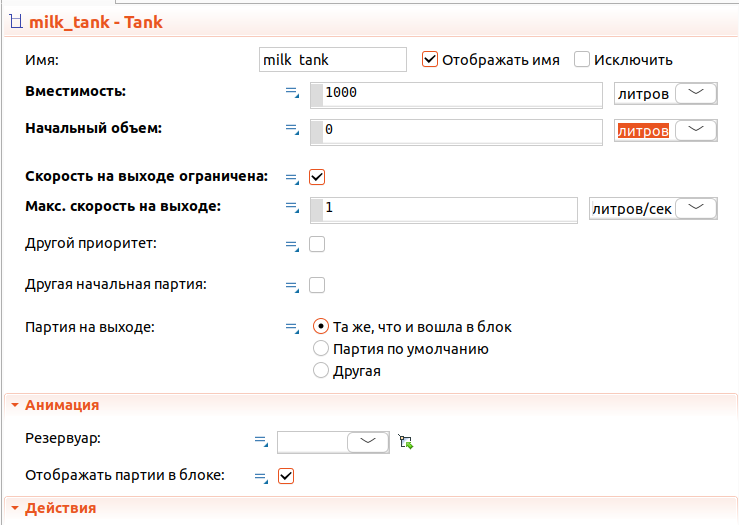
\includegraphics[scale=0.3]{fluid2}
	\caption{Блок \textit{Tank}}
	\label{fig:fluid2}
\end{figure}

Доставка жидких ингредиентов в смеситель осуществляется по трубам. Для моделирования трубопроводов используется \textit{Pipeline}. Также он моделирует трубу, по которой жидкость транспортируется из одной точки в другую. Имеет ограниченный объем. Есть опция, позволяющая содержать некоторое начальное количество жидкости на входе. (Рисунок \ref{fig:fluid3})
\begin{figure}[h]
	\centering 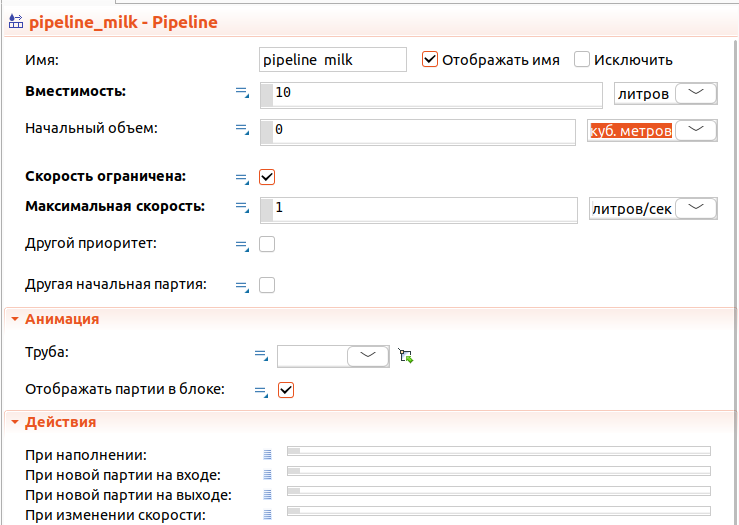
\includegraphics[scale=0.35]{fluid3}
	\caption{Блок \textit{Pipeline}}
	\label{fig:fluid3}
\end{figure}

Доставка масла выполняется по конвейеру. Для моделирования этого конвейера будем используется объект \textit{BulkConveyor}. Транспортирует объемные или конденсирующиеся летучие вещества из одной точки в другую. По сравнению с трубой \textit{Pipeline}, допускает образование зазоров и участков с различной "плотностью". Скорость потока на входе конвейера не обязательно равна скорости потока на его выходе. (Рисунок \ref{fig:fluid4})
\begin{figure}[h]
	\centering 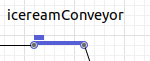
\includegraphics[scale=0.35]{fluid4}
	\caption{Блок \textit{BulkConveyor}}
	\label{fig:fluid4}
\end{figure}

\newpage

Процесс смешивания моделируется блоком \textit{MixTank}. У этого блока пять входов и один выход. На вход подаются ингредиенты в заданных пропорциях, на выходе -- смесь в заданных пропорциях. (Рисунок \ref{fig:fluid5})
\begin{figure}[h]
	\centering 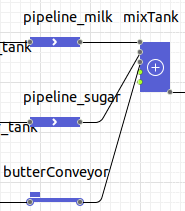
\includegraphics[scale=0.5]{fluid5}
	\caption{Блок \textit{MixTank}}
	\label{fig:fluid5}
\end{figure}

Поскольку смесь заморожена, то доставка ее осуществляется конвейером для конденсированных веществ. Порция мороженого -- это выделяемая из потока смеси заявка. Для процесса разделения на порции используем блок \textit{FluidToAgent}. (Рисунок \ref{fig:fluid6})
\begin{figure}[h]
	\centering 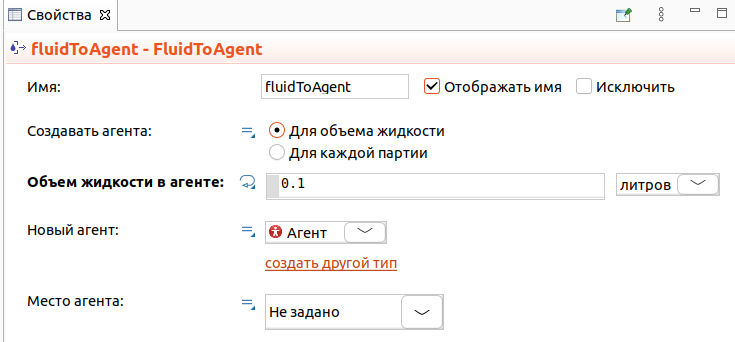
\includegraphics[scale=0.5]{fluid6}
	\caption{Блок \textit{FluidToAgent}}
	\label{fig:fluid6}
\end{figure}

Порции смеси должны помещаться в стаканчики. Для моделирования процесса появления стаканчиков будем использовать библиотеку моделирования процессов. Источник стаканчиков – блок \texit{Source}.  Поскольку скорость производства мороженого и стаканчиков в модели разная, то необходимы их накопители. Накопители моделируем блоком \textit{Queue}.\\

Сборка штучных заявок моделируется блоком \textit{Assembler}. Этот блок имеет пять входов и один выход. Он может принимать до пяти агентов и собирать из них нового агента. Первый вход блока - выход очереди мороженого, второй -- выход очереди стаканчиков. Моделирование доставки стаканчиков мороженого до упаковщика моделируется конвейером. Упаковка моделируется объектом \textit{Service}, в свойствах которого задается время процесса и его ресурсы. Ресурсы -- упаковщики. Упаковку мороженого промоделируем объектом \textit{Batch}, который собирает партии из входящих в него заявок. (Рисунок \ref{fig:fluid7})

\begin{figure}[h]
	\centering 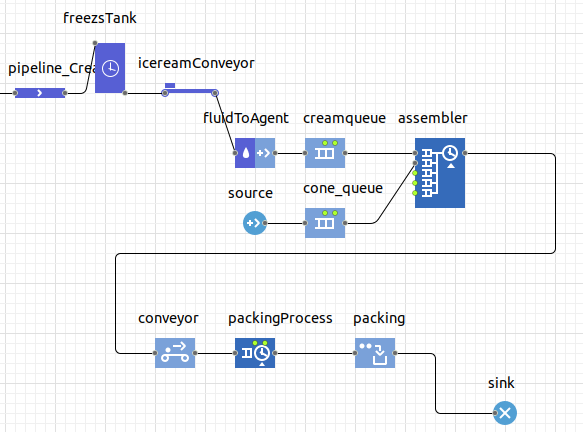
\includegraphics[scale=0.5]{fluid7}
	\caption{Процесс сборки, упаковки и отправки на склад стаканчиков с мороженным}
	\label{fig:fluid7}
\end{figure}

 Узкими местами модели являются блоки \textit{Tank}, однако, в связи с технологией производства мы не можем уменьшать время задержки в них, но можем  увеличить скорость работы конвейеров и скорость потока в трубах и в начальных блоках \textit{Tank}, тогда количество парий, отправленных на склад, увеличится. (Рисунок \ref{fig:fluid8})
 
 \begin{figure}[h]
 	\centering 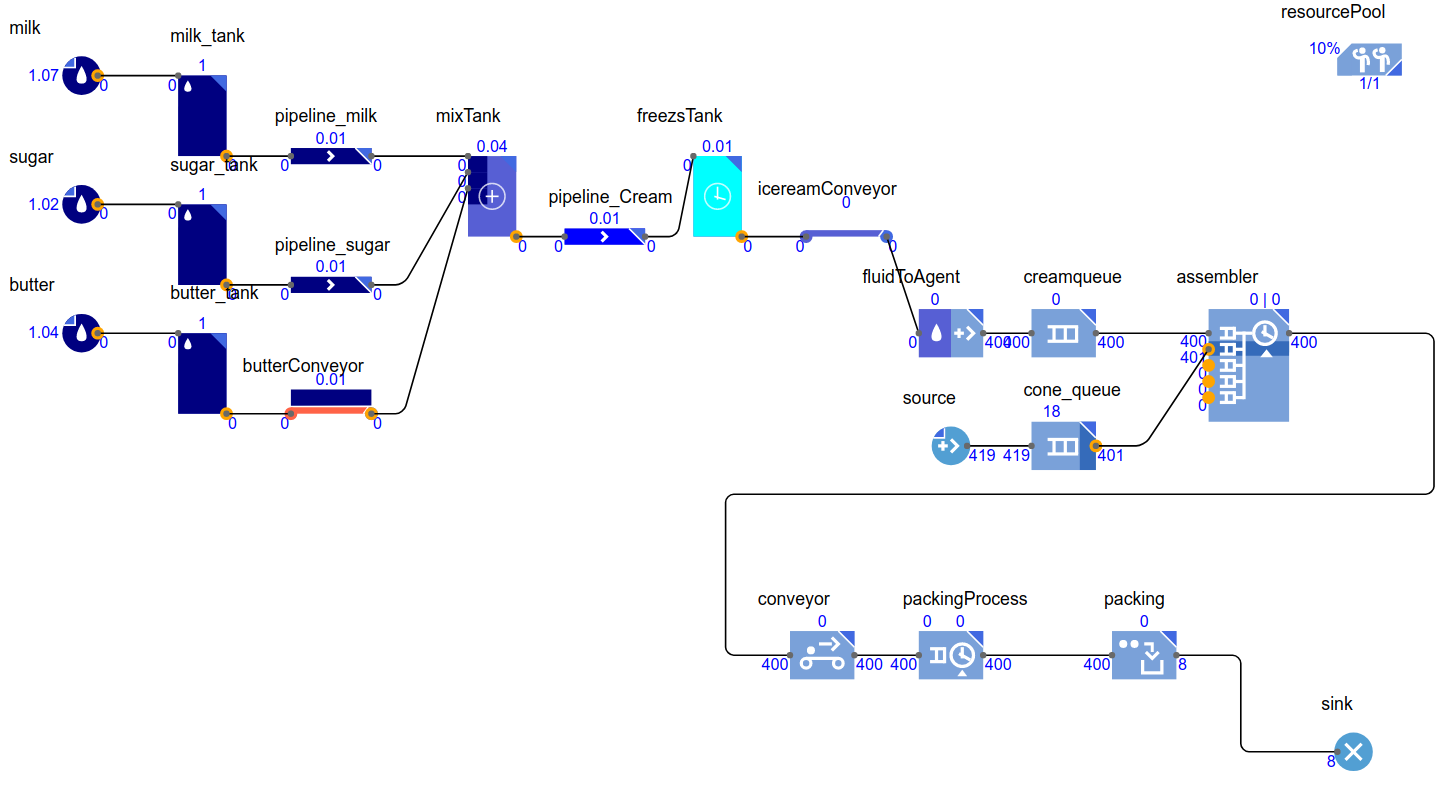
\includegraphics[scale=0.2]{fluid8}
 	\caption{Результат работы модели}
 	\label{fig:fluid8}
 \end{figure}

Таким образом, был промоделирован процесс производства мороженого.